\documentclass[11pt]{article}
\usepackage[margin=0.55in]{geometry}
\usepackage{amsmath,amssymb,booktabs,array,tabularx,multirow}
\usepackage{tikz}
\usetikzlibrary{arrows.meta,calc,decorations.pathreplacing,positioning}
\usepackage{xcolor}
\pagestyle{empty}

\newcommand{\mm}{\,\mathrm{mm}}
\newcommand{\degc}{^{\circ}}
\newcommand{\T}{\mathrm{T}}
\newcommand{\I}{\mathrm{I}}
\newcommand{\M}{\mathrm{M}}

\begin{document}

\begin{center}
{\Large \textbf{15-DoF Reconfigurable Three-Finger Hand: Kinematic Layout}}\\[2mm]
{\small Six XY morphology DoFs + nine finger articulation DoFs. The external 6-DoF palm pose used in the MuJoCo scene is not counted.}
\end{center}

\vspace{1mm}
\noindent
The CAD workspace drawing is registered to the MuJoCo palm frame by centering the overall CAD envelope at
$(55,80)\mm$ and rotating it so that the thumb opposes the other fingers along the MuJoCo $x$ direction:
\[
 x_{\rm MJ}=-(y_{\rm CAD}-80\mm),\qquad
 y_{\rm MJ}=-(x_{\rm CAD}-55\mm).
\]
Thus zero morphology places each finger at the center of its rectangular XY workspace.

\begin{center}
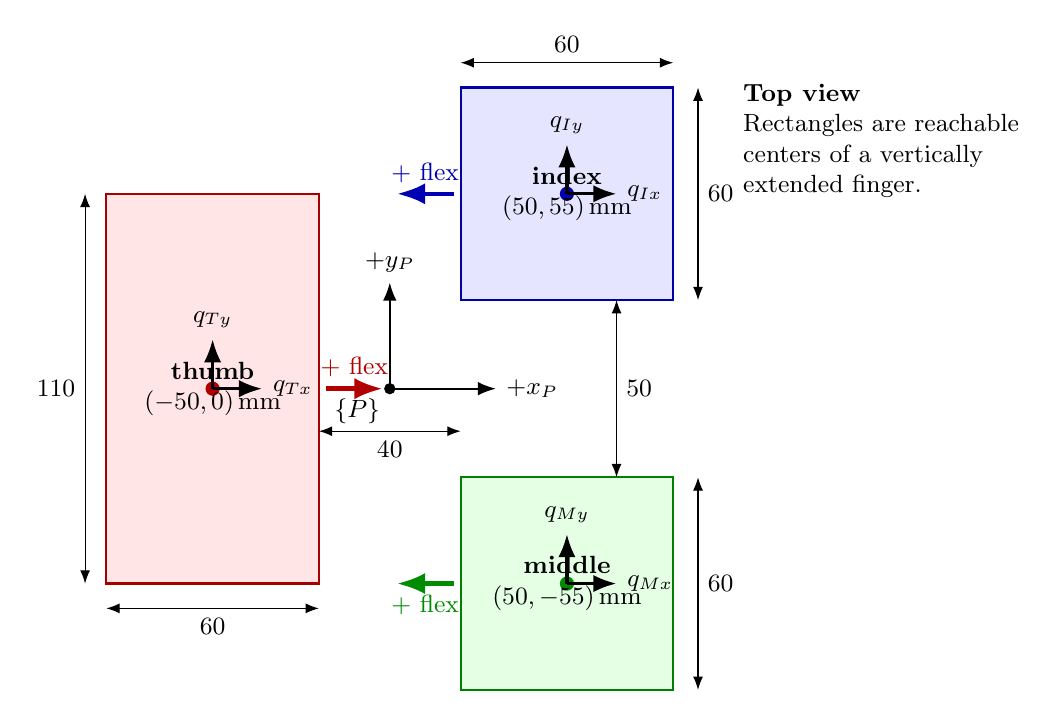
\begin{tikzpicture}[x=0.045cm,y=0.045cm,>=Latex,font=\small]
  % Workspace rectangles in MuJoCo XY coordinates, dimensions in mm.
  \filldraw[fill=red!10,draw=red!65!black,thick] (-80,-55) rectangle (-20,55);
  \filldraw[fill=blue!10,draw=blue!65!black,thick] (20,25) rectangle (80,85);
  \filldraw[fill=green!10,draw=green!50!black,thick] (20,-85) rectangle (80,-25);

  % Workspace centers.
  \fill[red!70!black] (-50,0) circle[radius=2.0];
  \fill[blue!70!black] (50,55) circle[radius=2.0];
  \fill[green!55!black] (50,-55) circle[radius=2.0];

  \node[align=center] at (-50,0) {\textbf{thumb}\\$(-50,0)\mm$};
  \node[align=center] at (50,55) {\textbf{index}\\$(50,55)\mm$};
  \node[align=center] at (50,-55) {\textbf{middle}\\$(50,-55)\mm$};

  % Morphology axes at each center.
  \foreach \cx/\cy/\lab in {-50/0/T,50/55/I,50/-55/M}{
    \draw[->,very thick] (\cx,\cy) -- ++(14,0) node[right] {$q_{\lab x}$};
    \draw[->,very thick] (\cx,\cy) -- ++(0,14) node[above] {$q_{\lab y}$};
  }

  % Palm frame origin and axes.
  \fill (0,0) circle[radius=1.6];
  \node[below left] at (0,0) {$\{P\}$};
  \draw[->,thick] (0,0) -- (30,0) node[right] {$+x_{P}$};
  \draw[->,thick] (0,0) -- (0,30) node[above] {$+y_{P}$};

  % Dimensioning: workspace sizes and gaps.
  \draw[<->] (-86,-55) -- (-86,55) node[midway,left] {$110$};
  \draw[<->] (-80,-62) -- (-20,-62) node[midway,below] {$60$};
  \draw[<->] (20,92) -- (80,92) node[midway,above] {$60$};
  \draw[<->] (87,25) -- (87,85) node[midway,right] {$60$};
  \draw[<->] (87,-85) -- (87,-25) node[midway,right] {$60$};
  \draw[<->] (-20,-12) -- (20,-12) node[midway,below] {$40$};
  \draw[<->] (64,-25) -- (64,25) node[midway,right] {$50$};

  % Opposing flexion directions at zero yaw.
  \draw[->,red!70!black,ultra thick] (-18,0) -- (-2,0) node[midway,above] {+ flex};
  \draw[->,blue!70!black,ultra thick] (18,55) -- (2,55) node[midway,above] {+ flex};
  \draw[->,green!55!black,ultra thick] (18,-55) -- (2,-55) node[midway,below] {+ flex};

  \node[align=left,anchor=west] at (97,70) {\textbf{Top view}\\
    Rectangles are reachable\\
    centers of a vertically\\
    extended finger.};
\end{tikzpicture}
\end{center}

\vspace{-2mm}
\begin{center}
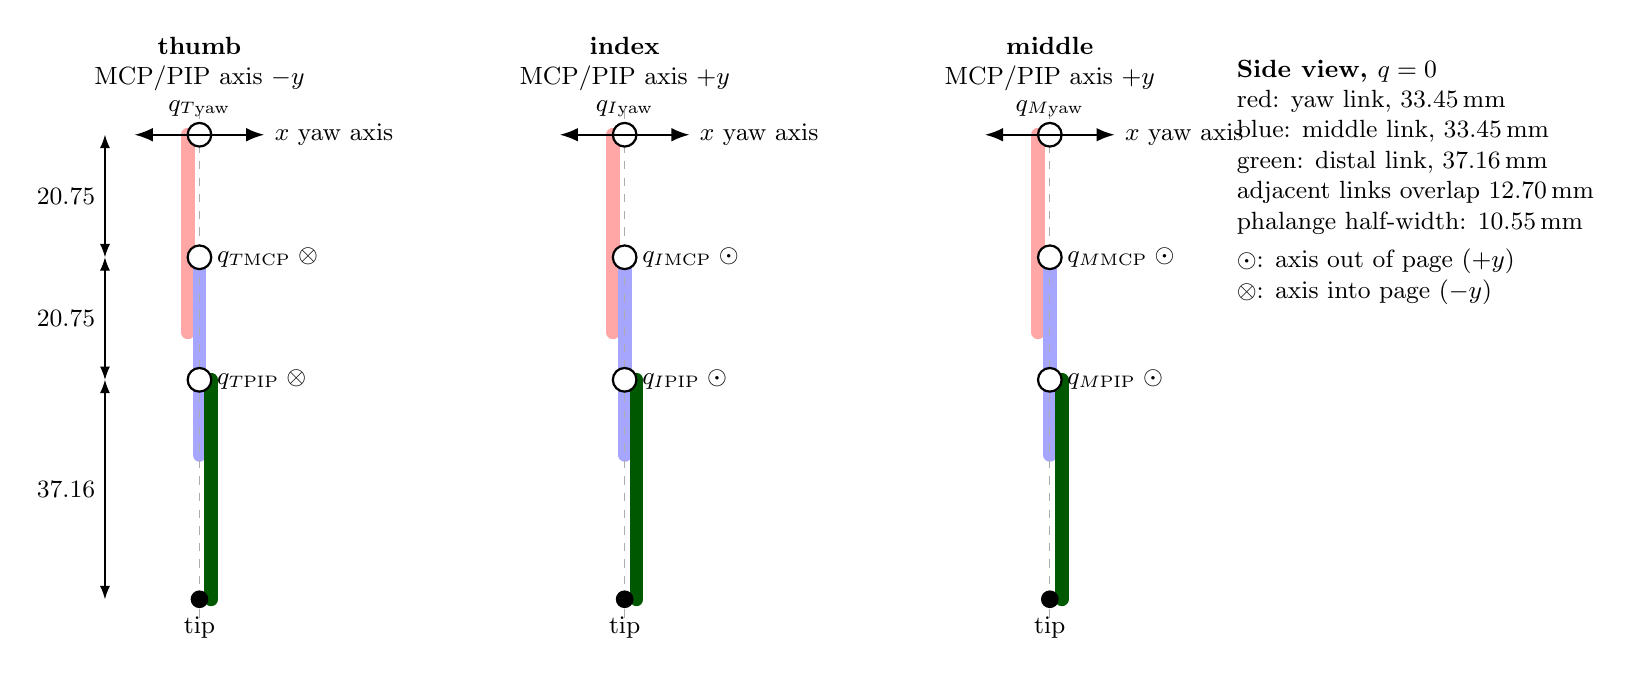
\begin{tikzpicture}[x=0.075cm,y=0.075cm,>=Latex,font=\small]
  % Helper macro: side-view chain. #1 x offset, #2 label, #3 hinge symbol, #4 flex direction text
  \newcommand{\fingerchain}[4]{%
    \begin{scope}[shift={(#1,0)}]
      % overlapping physical links, offset slightly in x so overlaps are visible
      \draw[line width=5pt,red!35,line cap=round] (-2,0) -- (-2,-33.45);
      \draw[line width=5pt,blue!35,line cap=round] (0,-20.75) -- (0,-54.20);
      \draw[line width=5pt,green!35!black,line cap=round] (2,-41.50) -- (2,-78.66);

      % centerline and joints
      \draw[gray!65,dashed] (0,4) -- (0,-82);
      \filldraw[fill=white,thick] (0,0) circle[radius=2.0];
      \filldraw[fill=white,thick] (0,-20.75) circle[radius=2.0];
      \filldraw[fill=white,thick] (0,-41.50) circle[radius=2.0];
      \fill (0,-78.66) circle[radius=1.5];

      \node[above=1mm] at (0,0) {$q_{#2\mathrm{yaw}}$};
      \node[right=1mm] at (0,-20.75) {$q_{#2\mathrm{MCP}}\;#3$};
      \node[right=1mm] at (0,-41.50) {$q_{#2\mathrm{PIP}}\;#3$};
      \node[below=1mm] at (0,-78.66) {tip};

      % yaw axis at base (x is in the page)
      \draw[<->,thick] (-11,0) -- (11,0) node[right] {$x$ yaw axis};
      \node[align=center] at (0,12) {#4};
    \end{scope}
  }

  \fingerchain{0}{T}{\otimes}{\textbf{thumb}\\MCP/PIP axis $-y$}
  \fingerchain{72}{I}{\odot}{\textbf{index}\\MCP/PIP axis $+y$}
  \fingerchain{144}{M}{\odot}{\textbf{middle}\\MCP/PIP axis $+y$}

  % Shared dimensions at left of first chain.
  \draw[<->] (-16,0) -- (-16,-20.75) node[midway,left] {$20.75$};
  \draw[<->] (-16,-20.75) -- (-16,-41.50) node[midway,left] {$20.75$};
  \draw[<->] (-16,-41.50) -- (-16,-78.66) node[midway,left] {$37.16$};

  \node[align=left,anchor=west] at (174,-8) {\textbf{Side view, $q=0$}\\
  red: yaw link, $33.45\mm$\\
  blue: middle link, $33.45\mm$\\
  green: distal link, $37.16\mm$\\
  adjacent links overlap $12.70\mm$\\
  phalange half-width: $10.55\mm$\\[1mm]
  $\odot$: axis out of page $(+y)$\\
  $\otimes$: axis into page $(-y)$};
\end{tikzpicture}
\end{center}

\vspace{1mm}
\section*{Morphology workspace parameters}
\begin{center}
\begin{tabular}{lrrrrrr}
\toprule
Finger & $x_0$ [mm] & $y_0$ [mm] & $q_x$ range [mm] & $q_y$ range [mm] & full workspace [mm] \\
\midrule
Thumb  & $-50$ & $0$   & $[-30,30]$ & $[-55,55]$ & $60\times110$ \\
Index  & $ 50$ & $55$  & $[-30,30]$ & $[-30,30]$ & $60\times60$ \\
Middle & $ 50$ & $-55$ & $[-30,30]$ & $[-30,30]$ & $60\times60$ \\
\bottomrule
\end{tabular}
\end{center}

\section*{Complete 15-DoF internal-joint parameter table}
For each finger $f\in\{T,I,M\}$, the first two joints translate the entire finger/yaw frame in the palm plane. The remaining three joints form the articulated finger chain. Axis directions below are given at the zero configuration in the palm frame.

\begin{center}
\small
\begin{tabular}{lllcl}
\toprule
Finger & DoF & Type / axis & Range & Home-frame location \\
\midrule
Thumb & $q_{Tx}$ & P, $+x_P$ & $[-30,30]\mm$ & \multirow{2}{*}{$(-50,0,0)\mm$} \\
      & $q_{Ty}$ & P, $+y_P$ & $[-55,55]\mm$ & \\
      & $q_{T\rm yaw}$ & R, $+x$ & $[-85,85]\degc$ & yaw center \\
      & $q_{T\rm MCP}$ & R, $-y$ & $[-15,92]\degc$ & $20.75\mm$ below yaw \\
      & $q_{T\rm PIP}$ & R, $-y$ & $[-18,92]\degc$ & $41.50\mm$ below yaw \\
\midrule
Index & $q_{Ix}$ & P, $+x_P$ & $[-30,30]\mm$ & \multirow{2}{*}{$(50,55,0)\mm$} \\
      & $q_{Iy}$ & P, $+y_P$ & $[-30,30]\mm$ & \\
      & $q_{I\rm yaw}$ & R, $+x$ & $[-85,85]\degc$ & yaw center \\
      & $q_{I\rm MCP}$ & R, $+y$ & $[-15,92]\degc$ & $20.75\mm$ below yaw \\
      & $q_{I\rm PIP}$ & R, $+y$ & $[-18,92]\degc$ & $41.50\mm$ below yaw \\
\midrule
Middle & $q_{Mx}$ & P, $+x_P$ & $[-30,30]\mm$ & \multirow{2}{*}{$(50,-55,0)\mm$} \\
      & $q_{My}$ & P, $+y_P$ & $[-30,30]\mm$ & \\
      & $q_{M\rm yaw}$ & R, $+x$ & $[-85,85]\degc$ & yaw center \\
      & $q_{M\rm MCP}$ & R, $+y$ & $[-15,92]\degc$ & $20.75\mm$ below yaw \\
      & $q_{M\rm PIP}$ & R, $+y$ & $[-18,92]\degc$ & $41.50\mm$ below yaw \\
\bottomrule
\end{tabular}
\end{center}

\section*{DH representation of each 3R finger subchain}
A classical DH table is most useful for the 3R articulated subchain; the two orthogonal base slides are represented directly as prismatic joints in the table above. One consistent standard-DH frame assignment is:

\begin{center}
\begin{tabular}{clcccc}
\toprule
$i$ & Joint & $\theta_i$ & $d_i$ & $a_i$ & $\alpha_i$ \\
\midrule
1 & yaw & $q_{f\rm yaw}$ & $0$ & $20.75\mm$ & $\sigma_f 90\degc$ \\
2 & MCP & $q_{f\rm MCP}$ & $0$ & $20.75\mm$ & $0\degc$ \\
3 & PIP & $q_{f\rm PIP}$ & $0$ & $37.16\mm$ & $0\degc$ \\
\bottomrule
\end{tabular}
\end{center}
where $\sigma_T=+1$ and $\sigma_I=\sigma_M=-1$ for this frame choice. The sign change reflects the reversed thumb flexion-axis convention. DH frame signs are not unique; the MuJoCo axis vectors in the 15-DoF table above are the authoritative implementation convention.

\paragraph{Physical-link geometry.}
The yaw and middle physical links are each $33.45\mm$ from rotational-axis center to their distal surface. Because the next joint center occurs $20.75\mm$ downstream, each pair overlaps by $33.45-20.75=12.70\mm$. The distal link is $37.16\mm$ from PIP axis to fingertip surface. The capsule radius is $10.55\mm$; consequently the MuJoCo capsule medial-axis endpoints are $22.90\mm$, $22.90\mm$, and $26.61\mm$ so that the rounded surfaces terminate at the measured CAD dimensions.

\end{document}
